\newcommand{\grouprec}{\kw{batch}}
\newcommand{\optgrouprec}{\kw{batch}}
%\newcommand{\grouprecopt}{\kw{kTeamFormOpt}}
\newcommand{\minp}{\kw{minP}}
\newcommand{\rgraphsim}{\kw{undirgSim}}
\newcommand{\incsim}{\kw{incSim}}


\section{Dynamic Team Formation}
\label{sec-tsim}


We first propose {\em team simulation}, a revision of traditional graph pattern matching.
We then formally introduce the {\em top-$k$ team formation} problem via team simulation.
We finally present the {\em dynamic top-$k$ team formation} problem.

\eat{
In this section, we first present basic notations of graphs, and then propose team simulation, an extension of traditional graph pattern matching.
We finally formally introduce the top-$k$ team formation problem via team simulation, and propose a cubic algorithm with two optimization techniques.

\subsection{Data Graphs and Pattern Graphs}
\label{subsec-graphdefs}


\stitle{Data graphs}.
A {\em data graph} is a labeled undirected graph $G(V, E, l)$, where
(1) $V$ is a finite set of nodes;
(2) $E \subseteq V \times V$, in which $(u, u')$ or $(u', u)$ $\in E$ denotes an undirected edge between nodes $u$ and $u'$; and
(3) $l$ is a total labeling function that maps each node in $V$ to a set of labels.

%; and(4) $w$ is a total weight function that maps each edge in $E$ to a positive rational number.

Intuitively, the node labels carry the content of the node, \eg skills, keywords, blogs, rating~\cite{AmerYahiaBB07}.
The edges specify the affinity or collaborative compatibility among nodes~\cite{GajewarS12}.

\stitle{Pattern graphs}.
A {\em pattern graph} (or simply pattern) is an undirected graph $P(V_P$, $E_P$, $l_P$, $f_P)$, in which
(1) $V_P$ and $E_P$ are the set of nodes and the set of edges, respectively;
(2) $l_P$ is a total labeling function that maps each node in $V_P$ to a single label; and
(3) $f_P$ is a total capacity function such that for each node $u\in V_P$, $f_P(u)$ is a closed interval $[x, y]$, where $x\le y$ are non-negative integers.

Intuitively, $f_P(u)$ specifies a range bound for node $u$,
indicating the required quantity for the matched nodes in data graphs.
Note that for traditional graph patterns~\cite{Galla06, b-matching,FanLMTWW10,FanCount16}, bounds are typically carried on edges, not on nodes.
\looseness=-1


\begin{example}
\label{exm-pattern}
Consider pattern graph $P_1$ and data graph $G_1$ in Fig.~\ref{exm-motivation}. Observe that there is a capacity bound on each node in $P_1$.
For example, capacity bound [1,2] on node \kw{SD} in $P_1$ indicates in the match result,
there should be at least one and at most two nodes matched with \kw{SD}.
\end{example}


\stitle{Remarks}. We assume \kwlog~that pattern graphs are connected, as a common practice.
We also simply denote data graphs $G(V, E, l$) as  $G(V, E)$ and pattern graphs $P(V_P$, $E_P$, $l_P$, $f_P)$ as $P(V_P$, $E_P)$, respectively.
Furthermore, the size $|G|$ of data graphs $G$ (resp. $|P|$ of pattern graphs $P$) is the total number of nodes and edges in $G$ (resp. $P$).
}%%%EAT

\eat{%%%%%%%%%%%%%%%%
We shall use the following notation
	
\etitle{Subgraphs}.
Graph $H(V_s, E_s,  l_{H})$ is a {\em subgraph} of data graph $G(V, E, l)$, denoted as $G[V_s, E_s]$, if
(1) for each node $u\in V_s$, $u\in V$ and $l_{H}(u) = l(u)$, and
(2) for each edge $e\in E_s$, $e\in E$. % and $w_{H}(e) = w(e)$.
That is, subgraph $G[V_s, E_s]$ only contains a subset of nodes and a subset of edges of graph $G$.

We also denote subgraph $G[V_s, E_s]$ as subgraph $G[V_s]$, if $E_{s}$ is exactly


Similarly, we can define {\em subgraphs for pattern graphs}, which further requires the preservation of the node capacity.

\etitle{Induced subgraphs}. An {\em induced subgraph} $G_{s}(V_{s}, E_{s})$ is composed of vertices $V_{s}$ who is a subset of the vertices $V$ of graph $G(V, E)$, and together with the edge set $E_{s}$ whose endpoints are both in $V_{s}$ in $G(V, E)$.


\etitle{Subpatterns}.
Pattern $Q(V_s, E_s,  l_{q}, f_{q})$ is a {\em subpattern} of pattern $P(V_p$, $E_p$, $l_p$, $f_p)$, denoted as $P[V_s, E_s]$, if
(1) for each node $u\in V_s$, $u\in V$, $l_{q}(u) = l_p(u)$ and $f_{q}(u) = f_p(u)$, and
(2) for each edge $e\in E_s$, $e\in E$. % and $w_{H}(e) = w(e)$.
That is, subpattern $G[V_s, E_s]$ only contains a subset of nodes and a subset of edges of pattern $P$.}

% \etitle{Connected components}.
% A {\em connected component} of a graph is a subgraph in which any two nodes are connected to each other by undirected paths,
% and which is only connected to the nodes of itself, \ie a connected component is maximal.
% A graph that is itself connected has exactly one connected component, which is the entire graph.

\eat{%%%%%%%%%%%
\etitle{Neighbors}. We say that node $u'$ is a {\em neighbor} of node $u$ if there is an edge between $u$ and $u'$ in a data or pattern graph.

\etitle{Paths}.
A {\em simple path} (or simply a {\em path}) $\rho$ is a sequence of nodes $v_1/\ldots/v_n$ with no repeated nodes, and, moreover, for each $i\in[1, n-1]$, $(v_i$, $v_{i+1})$ is an edge in $G$. The {\em length} of a path $\rho$ is the number of edges in $\rho$.

A graph is {\em connected} if for each pair of nodes, there exists a  path connecting them.

\etitle{Distances}. Given two nodes $v$ and $v'$ in a graph $G$, the {\em  distance} from $v$ to $v'$,
denoted by $\dist(v,v')$, is  the shortest length of all {\em paths}
from $v$ to $v'$ in $G$.
}


\eat{%%%%%%%%%%
\etitle{Diameter}. The {\em diameter} of a connected graph $G$,  denoted by $\diameter{G}$, is the longest shortest distance of all pairs of nodes in $G$, \ie $\diameter{G}$ = $\kw{max}(\kw{dis}(v,v'))$ for all nodes $v,v'$ in $G$.
}%%%%%%%%%%%%%%


\eat{
\etitle{Distances}. The {\em length} of a path $\rho$ is
the sum of the weights of its constituent edges, \ie $\sum_{i=1}^{n-1} w(v_i, v_{i+1})$.

Given two nodes $v, v'$ in a graph $G$, the {\em distance} from $v$ to $v'$,
denoted by $\dist(v,v')$, is the length of the shortest {\em path}
from $v$ to $v'$ in $G$.
}

%\vspace{-4ex}
\subsection{Team Simulation}
\label{subsec-extsim}

We first extend pattern graphs of traditional graph pattern matching to carry capacity requirements,
and then define team simulation on undirected graphs.
%We then redefine strong simulation on directed graphs, originally defined on directed graphs~\cite{MaCFHW14}.}

We start with basic notations.

\stitle{Data graphs.} A {\em data graph} is a labeled undirected graph $G(V$, $E$, $l)$, where $V$ and $E$ are the sets of nodes and edges, respectively; and $l$ is a total labeling function that maps each node in $V$ to a set of labels.

\stitle{Pattern graphs}.
A {\em pattern graph} (or simply pattern) is an undirected graph $P(V_P$, $E_P$, $l_P$, $f_P)$, in which
(1) $V_P$ and $E_P$ are the set of nodes and the set of edges, respectively;
(2) $l_P$ is a total labeling function that maps each node in $V_P$ to a single label; and
(3) $f_P$ is a total capacity function such that for each node $u\in V_P$, $f_P(u)$ is a closed interval $[x, y]$, where $x\le y$ are non-negative integers.

Intuitively, $f_P(u)$ specifies a range bound for node $u$,
indicating the required quantity for the matched nodes in data graphs.
Note that for traditional patterns~\cite{Galla06, b-matching,FanLMTWW10,FanCount16}, bounds are typically carried on edges, not on nodes.
We also also denote data and pattern graphs as $G(V$, $E)$ and $P(V_{P}$, $E_{P})$ respectively. The size of $G$ (resp. $P$), denoted by $|G|$ (resp. $|P|$), is defined to be the total number of nodes and edges in $G$ (resp. $P$).

%We define $r$-simulation by extending graph simulation~\cite{infsimu95,FanLMTWW10,MaCFHW14} on undirected graphs  and introducing capacity constraints.

\eat{As strong simulation is an extension of graph simulation, which is also defined on directed graphs~\cite{infsimu95,FanLMTWW10},
We now redefine graph simulation on undirected graphs. Consider a pattern graph $P(V_P$, $E_P)$ and a data graph $G(V$, $E)$.
}%%%EAT

We now redefine graph simulation on undirected graphs, which is originally defined on directed graphs~\cite{infsimu95,FanLMTWW10}. Consider pattern graph $P(V_P$, $E_P)$ and data graph $G(V$, $E)$.


\stitle{Graph simulation}. Data graph $G$ {\em matches} pattern graph $P$ via
graph simulation, denoted by $P \eps G$, if there exists a binary {\em match relation} $\Reps \subseteq V_P \times V$ in $G$ for $P$ such that

\vspace{0.5ex}
\ni
(1) for each $(u, v) \in \Reps$, the label of $u$ matches one label in the label set of $v$, \ie $l_{P}(u) \in l(v)$; and

\vspace{0.5ex}
\ni
(2) for each node  $u\in V_P$, there exists $v\in V$ such that
(a) $(u, v) \in \Reps$, and
(b) for each adjacent node $u'$ of $u$ in $P$, there exists a adjacent node $v'$ of $v$
in $G$ such that $(u',v') \in \Reps$.

For any $G$ that matches $P$, there exists a {\em unique maximum} match relation via graph simulation~\cite{infsimu95}.

We then introduce the notions of balls and match graphs.

%While there may be multiple match relations in a graph $G$ for a pattern graph $P$,
%there exists a unique {\em maximum} match relation $\Reps_m$ in $G$ for $P$ such that for any match relation $R$ in $G$ for $P$, $\Reps \subseteq \Reps_m$,

\eat{%%%EAT
Intuitively, graph simulation preserves the label match and
neighborhood relationships between pattern graphs and the matched data graphs~\cite{FanLMTWW10,MaCFHW14}.

Following from \cite{FanLMTWW10,MaCFHW14}, the revised graph simulation above is well-defined, as shown below.
%Following from \cite{FanLMTWW10,MaCFHW14}, it is easy to know that the graph simulation revised above has the following.

\begin{prop}
\label{prop-sim-maximum-match}
For any data graph $G$ and pattern graph $P$  such that $P\eps G$, via graph simulation, there is a unique maximum match relation in $G$ for $P$.
\end{prop}
}%%%EAT


\etitle{Balls}. For a node $v$ in data graph $G$ and a non-negative integer $r$,
the {\em ball} with {\em center} $v$ and {\em radius} $r$  is a subgraph of $G$,
denoted by $\ball{[v, r]}$, such that (1) all nodes $v'$ are in $\ball{[v, r]}$, if
the number of hops between $v'$ and $v$, $\hop(v', v)$, is no more than $r$, and (2) it has exactly the edges
appearing in $G$ over the same node set.

\eat{%%EAT
Intuitively, a ball is a connected graph such that all node pairs have bounded hops.
Indeed, as observed in~\cite{Buchan2004}, when social distance increases, the
closeness of relationships decreases and the  relationships may become
irrelevant. Hence it often suffices in practice to consider only those
matches of a pattern graph that fall in a small ball.
}%%%EAT

\etitle{Match graphs}. The {\em match} graph $\wrt$ a binary relation $\Reps\subseteq V_P\times V$ is a subgraph $G_s$ of data graph $G$, in which
(1)  a node $v\in V_s$ if and only if it is in $\Reps$, and
(2) it has exactly the edges
appearing in $G$ over the same node set.

Intuitively, the match graph $G_s$ $\wrt$ $\Reps$ is the induced subgraph of
$G$ such that its nodes play a role in $\Reps$.


\eat{%%%%EAT
\stitle{Induced match graphs}. Consider a binary relation $\Reps\subseteq V_q\times V$.
The {\em induced match} graph $\wrt$ $\Reps$ is a induced subgraph $G[V_s, E_s]$ of $G$, in which
(1) a node $v\in V_s$ if and only if it is in $\Reps$, and
(2) an edge $(v,v')\in E_s$ if and only if $v$ and $v'$ are in $\Reps$.
%
Intuitively, the induced match graph $G[V_s, E_s]$ $\wrt$ $\Reps$ is the induced subgraph of $G$ such that each of its nodes plays a role in $\Reps$, together with the adjacent edges in $G$.
}%%%%%%%%%EAT

We are now ready to define team simulation, by extending graph simulation to incorporate the locality constraints enforced by balls, and the capacity bounds carried by patterns.
\looseness=-1

%\vspace{-1ex}
\stitle{Team simulation}. Data graph $G$ {\em matches} pattern $P$  via
team simulation \wrt a radius $r$, denoted by $P \eeps G$, if
there exists a {\em ball} $\ball{[v, t]}$ ($t \in [1,r]$, $t \in Z$) in $G$, such that

\vspace{0.5ex}
\ni(1) $P\eps \ball{[v, t]}$, with the maximum match relation $\Reps$ and the match graph $G_s$ $\wrt$ $\Reps$; and

\vspace{0.5ex}
\ni(2) for each node $u$ in $P$, the number of nodes $v$ in $G_s$  with $(u, v)\in \Reps$ falls into $f_P(u)$.

\vspace{0.5ex}
We refer to  $G_s$ as a {\em perfect} subgraph of $G$ \wrt $P$.


Intuitively, (1) pattern graphs $P$ capture the structural and capacity constraints, and (2) a perfect subgraph $G_s$ of pattern $P$ corresponds to a desired team, which is required to satisfy the following conditions:
(a) $G_s$ itself is located in a ball $\ball{[v, t]}$  where $t \in [1,r]$ as a match graph; and
(b) $G_s$ satisfies the capacity constraints carried over pattern $P$.



\begin{example}
\label{exm-rsimulation}
Consider pattern $P_1$ and data graph $G_1$ in Fig.~\ref{exm-motivation}, and  team simulation with $r=2$ is adopted.

One can easily verify that $P_1$ matches $G_1$  via team simulation, \ie $P_1 \eeps G_1$,
as (a) there is a perfect subgraph in in ball
$\ball{[\kw{PM_1}, 2]}$, \ie the connected component of $G_1$ containing $\kw{PM_{1}}$, which maps \kw{PM}, \kw{BA}, \kw{UD}, \kw{SA}, \kw{SD} and \kw{ST} in $P_1$ to \kw{PM_1}, \kw{BA_1}, \{\kw{UD_1}, \kw{UD_2}\}, \{\kw{SA_1}, \kw{SA_2}\}, \{\kw{SD_1}, \kw{SD_2}\} and \{\kw{ST_1}, \kw{ST_2}\}, respectively, and, moreover, (b) the capacity bounds on all pattern nodes are satisfied.
\end{example}

\eat{%%%170720
\stitle{Remarks}.
(1) Graph simulation is a special case of team simulation on undirected graphs,
when the capacity on each pattern node is $[1, +\infty]$, and $r$ is no less than the diameter of data graphs.
%
(2) Further, strong simulation is also a special case of team simulation on undirected graphs,  when the capacity on each pattern node is $[1, +\infty]$,
$r$ is equal to the diameter of pattern graphs, and match graphs only involve with those edges matching edges in pattern graphs.
}%%%EAT170720

\vspace{-1ex}
\stitle{Remarks}.
(1) Team simulation differs from graph simulation~\cite{infsimu95} and strong simulation~\cite{MaCFHW14} in the existence of capacity bounds on pattern graphs and its ability to capture matches on undirected graphs.

\sstab(2) Different from strong simulation with a fixed radius for balls (\ie the diameter of a pattern), team simulation adopts a more natural setting that the radius of balls is auto-adjustable, having a user specified upper bound only.

%(2) Graph simulation (resp. strong simulation) is a special case of team simulation on undirected graphs when the capacity on each pattern node is $[1, +\infty]$, and $r$ is no less than (resp. equal to) the diameter of data graphs (resp. pattern graphs).





\eat{%%%EAT
\stitle{Remarks}.
(1) Graph simulation is a special case of (1) team simulation for undirected graphs,
when the capacity on each pattern node is $[1, +\infty]$ and $r$ is no less than the diameter of data graphs.
%
(2) Graph simulation~\cite{FanLMTWW10} and dual simulation~\cite{MaCFHW14} are equal on undirected graphs.
Hence, many good properties of dual simulation naturally carry over to graph simulation on undirected graphs.
%
(3) {\bf The difference of matched graphs between strong simulation and T-simulation.}
}%%%EAT

%and also a special case of (2) subgraph isomorphism, when the labels on pattern nodes are different from each other and the capacity on each pattern node is $[1, 1]$.

%(1) Graph simulation and its extensions were originally proposed on directed graphs.
%They were introduced for social networks analysis~\cite{BrynielssonHKMS10}, and for graph pattern matching~\cite{FanLMTWW10,FanLMTW11} due to its low \PTIME
%computational complexity~\cite{infsimu95}.


\eat{%%%%%%%%

When given a pattern graph, we first make a examination on it ensuring that there exist data graphs in which we can find matches using the pattern graph. If the answer is true, we can execute the following computing work. Otherwise, we require the user to retype in another pattern graph.
}


\eat{%%%170720
\begin{figure}[tb!]
%\vspace{-1ex}
\begin{center}
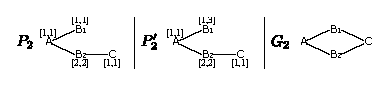
\includegraphics[scale=1.28]{./fig/consistency_motivation.eps}
\end{center}
\vspace{-3ex}
\caption{Pattern graphs}
\vspace{-4ex}
\label{fig-consistency-example}
\end{figure}

\stitle{Pattern satisfiability}.
We say that a pattern $P$ is {\em satisfiable} iff there exists a data graph $G$ such that $P \eeps G$.



Different from graph simulation \cite{infsimu95} and its extensions \cite{FanLMTWW10,MaCFHW14},
pattern graphs may be unsatisfiable for team simulation, due to the presence of capacity constraints enforced on patterns. We illustrate this with an example below.
%\looseness=-1

\begin{example}
\label{exm-consistency}
\ni(1)  Consider pattern $P_2$ in Fig.~\ref{fig-consistency-example}.
One can verify that there exist no data graphs $G$ such that $P_2 \eeps G$ because (a) for any nodes $u$ in $G$, if $u$ matches with the node labeled with $B_2$, then it must match with the node labeled with $B_1$, and, hence, (b) the capacity upper bound on $B_1$ should not be less than the lower bound on $B_2$.


\sstab(2) Pattern $P_1$ in Fig.~\ref{exm-motivation} is satisfiable as $P_1 \eeps G_1$.
\end{example}


The good news is that checking the satisfiability of pattern graphs can be done in low polynomial time.

\begin{prop}
\label{prop-pattern-consistency}
The satisfiability of patterns $P$ can be checked in $O(|P|^2)$ time.
\end{prop}

\proofS By treating $P$ as both data and pattern graphs, compute the maximum match relation $M$ in $P$ for $P$, via graph simulation.
Indeed, pattern $P$ is satisfiable iff for each $(u, v)\in M$ with the capacity bounds $[x_u, y_u]$ on $u$ and $[x_v, y_v]$ on $v$, respectively, $x_v \leq y_u$ holds. Observe that the size of $M$ is bounded by $|P|^2$.
\eop

Pattern graphs are typically small, and we only consider  satisfiable patterns in the sequel, by Proposition~\ref{prop-pattern-consistency}.
}

\subsection{Top-k Team Formation}
\label{subsec-teamF}

 Given pattern $P$, data graph $G$, and two positive integers $r$ and $k$, the {\em top-$k$ team formation} problem, denoted as \teamF{(P, G, k)},
is to find a list $L_{k}$ of $k$ perfect subgraphs (\ie teams) with the top-$k$ largest density in $G$ for $P$, via team simulation.
\looseness=-1

Here the {\em density}\, $\density{G}$ of graph $G(V, E)$ is $|E|/|V|$, where $|E|$ and $|V|$ are the number of edges and the number of nodes respectively, as commonly used in data mining applications~\cite{maximumDenseSubgraph,EVMK12}.
Intuitively, the larger $\density{G}$ is, the more collaborative a team is.
In this way, not only the two objective functions of existing team formation methods are preserved,
\ie the locality retained by balls and the density function in selecting top-$k$ results,
but also the relationships among members and the capacity constraint on patterns.


\begin{example}
\label{exa-teamF}
Consider $P_1, G_1$ in Fig.~\ref{exm-motivation} and $r=2$.
We simply set $k=1$, as most existing solutions for \teamF{} only compute the best team \cite{Lappas09,ArisLuca12,GajewarS12,realTeamForm13,SamikKVM12}.

One may want to look for candidate teams with existing methods, satisfying the search requirement in Example \ref{exm-motivation}:
\ni(1) by minimizing the {\em team diameter} \cite{Lappas09},
which returns the team with $\{\kw{BA_3}$, \kw{PM_3}, \kw{UD_4}, \kw{SA_4}, \kw{SD_4}, $\kw{ST_4}\}$,

\ni(2) by minimizing the {\em sum of all-pair distances} of teams \cite{Kargar11},
which returns exactly the same team as (1) in this case, or

\ni(3) by maximizing the {\em team density} \cite{GajewarS12}, which returns the team with all the nodes in the two connected components in $G_1$ with \kw{PM_1} and \kw{BA_3}, except \kw{UD_2}, \kw{PM_3}, \kw{UD_4}, \kw{SA_4}.

One may already notice that these teams only satisfy the skill requirement, \ie condition (i) in Example \ref{exm-motivation}, and cannot guarantee  the specific collaboration relationships among team members.
Indeed, the team found in (1) and (2) is connected by \kw{BA_3} only, and the team found in (3) has loose collaborations among its members.
That is, existing methods are not appropriate for identifying the the desired teams.

When team simulation is adopted, it returns the perfect subgraph in Example \ref{exm-rsimulation} with its density = 1.4,
satisfying both conditions (i) and (ii), much better than those teams found by the above existing methods.
\end{example}

\eat{%%%EAT
\sstab
(a) Algorithm \mindia~\cite{Lappas09} is to find a team with the {\em minimum diameter}, and returns $\{\kw{BA_3}$, \kw{PM_3}, \kw{UD_4}, \kw{SA_4}, \kw{SD_4}, $\kw{ST_4}\}$.

\sstab
(b) Algorithm \minsumdis~\cite{Kargar11} aims at minimizing the sum of all-pair distances, which is an extension of \mindia, and it returns exactly the same team as \mindia in this case.

\sstab
(c) Algorithm \denalk~\cite{GajewarS12} is to find a team with the {\em largest density}, and
returns the subgraph consisting of the two connected components of $G_1$ containing \kw{PM_1} and \kw{BA_3} respectively (excluding \kw{UD_1},\kw{PM_3},\kw{UD_4},\kw{SA_4}), whose density is 1.5.
%Indeed, larger density always results in a larger quantity.

\sstab
(d) Our team simulation returns the perfect subgraph in Example \ref{exm-rsimulation} with its density = 1.4 as the best team.

One can see that only team simulation captures the topology, cardinality and collaboration requirements of teams.
}%%%EAT



\eat{%%%EAT170720
\begin{figure}[t!]
%\vspace{-2ex}
\begin{center}
{\small
\myhrule
\vspace{-3ex}
\mat{0ex}{
\sstab {\sl Input:\/} $G(V$, $E)$, $P(V_P$, $E_P)$, and positive integers $k, r$.\\
{\sl Output:\/} The list $L_{k}$ of top-$k$ teams\\
\sstab \bcc \hspace{1ex} \= $L_{k} := \emptyset$;\\
\icc \> \For each ball $\ball{[v,r]}$ in $G$ \Do\\
\icc \>\hspace{2ex}\= $G_s$ := \rgraphsim$(P, \ball{[v,r]})$;\\
\icc \>\> \If $\density{G_s}>$ the density of the $k$-th result in $L_{k}$ \Then\\
%\icc \>\> \If $\density{G_s}>$ the density of $kth$ result in $L_{k}$ and there exists\\
%     \>\>\hspace{0.5ex}   no $G'_s$ in $L_{k}$ that is same with $G_{s}$ \Then\\
\icc \>\>\hspace{2ex}\= remove the $k$-th result in $L_{k}$ and insert $G_s$ into $L_{k}$;\\
\icc \> \Return $L_{k}$.
}

\vspace{-4ex} \myhrule
}
\end{center}
\vspace{-3ex}
\caption{Algorithm \grouprec} \label{alg-grouprec}
\vspace{-4ex}
\end{figure}

We now present an algorithm for \teamF{} via team simulation.


\stitle{Algorithm for Top-k Team Formation.} Given $P$, $G$, and two integers $r$ and $k$, an algorithm, referred to as \grouprec, is shown in Fig.~\ref{alg-grouprec}.
\grouprec is to find the set of perfect subgraphs $G_s$ by inspecting those balls $\ball{[v, r]}$ centered at each node $v$ of $G$, and returns the top-$k$ densest ones.
It computes the perfect subgraph $G_s$ of $P$ in the ball $\ball{[v,r]}$ via team simulation by invoking \rgraphsim(lines 2-3).
Procedure \rgraphsim is deferred to the appendix, which is an adaption from graph simulation~\cite{infsimu95,FanLMTWW10},
by extending from directed to undirected graphs,  incorporating the capacity constraint check, and only maintaining the capacity bounds satisfied perfect subgraphs.
In the process, \grouprec maintains the top-$k$ non-repeated perfect subgraphs with current top-$k$ largest density (lines 4-5), and returns them when all balls are processed (line 6).


\begin{example}
\label{exa-alg-batch} Consider $r=2$ and $k=2$.

\sstab(1) For $P_1$ and $G_1$ (ignore dashed edges) in Fig.~\ref{fig-motivation-example},
 \grouprec returns the team found in Example~\ref{exm-rsimulation} as its only answer.

\sstab(2) For $P_1$ and $G_1$ (with dashed edges), \grouprec returns the team in (1) as the best,
and the connected component containing \kw{PM_2} with its density = 1 as the second best.
\end{example}


\stitle{Correctness \& complexity analyses}. The correctness of algorithm \grouprec is assured by the following.
(1) There is a unique perfect subgraph in each ball of $G$.
(2) The correctness of \rgraphsim can be verified along the same lines as for simulation~\cite{infsimu95}.
(3) The list $L_{k}$ always maintains the current top-$k$ teams with largest density.
It takes $O(|V||P||G|)$ time to compute team simulation for all balls,
and $O(|V|\cdot(|V_{G_s}|^2+|G_s|))$ time to maintain the top-$k$ teams.
Thus \grouprec is in $O(|V|\cdot(|P||G|+|V_{G_s}|^2))$ time.
}%%%EAT170720


\subsection{Dynamic Top-k Team Formation}
\label{subsec-dynteamF}

We now introduce dynamic top-$k$ team formation.
%For convenience, the notations used are summarized in Table~\ref{tab-notation}.

\stitle{Pattern updates ($\Delta P$)}. There are five types of pattern updates:
%
(1) {\em edge insertions} connecting nodes in $P$,
%
(2) {\em edge deletions} disconnecting nodes in $P$,
%
(3) {\em node insertions} attaching new nodes to $P$,
%
(4) {\em node deletions} removing nodes from $P$, and
%
(5) {\em capacity changes} adjusting the node capacities in $P$,
%
while $P$  remains connected in all cases.


\stitle{Data updates ($\Delta G$)}. There are four types of data updates,
defined along the same lines as the first four types of pattern updates.
Further, different from pattern updates, there is no need to keep $G$ connected for data updates.


\stitle{Dynamic top-$k$ team formation}. Given pattern $P$, data graph $G$, positive integers $r$ and $k$, the list $L_{k}(P,G)$ of top-$k$ perfect subgraphs for $P$ in $G$,
a set of pattern updates $\Delta P$ and a set of data updates $\Delta G$,
the {\em dynamic top-k team formation} problem, denoted by \dynteamF{(P, G, k, L_{k}, \Delta P, \Delta G)},
is to find a list of $k$ perfect subgraphs with the top-$k$ largest density for $P\oplus\Delta P$ in $G\oplus\Delta G$, via team simulation.


Here $\oplus$ denotes applying changes $\Delta P$ to $P$ and $\Delta G$ to $G$, and
 $P\oplus\Delta P$ and $G\oplus\Delta G$ denote the updated pattern and data graphs.
 It is worth mentioning that \dynteamF{} covers a broad range of dynamic situations,
\ie handling continuously separate and simultaneous pattern and data updates.

\eat{
\begin{example}
\label{exm-dyn-team}
Recall $P_1$, $G_1$, $\Delta P_1$ and $\Delta G_1$ in Example \ref{exm-motivation-inc} (3), and set $r=2$ and $k=2$.
When get the top-$2$ teams for $P_1$ in $G_1$, \ie $L_k(P_1,G_1)$,
\dynteamF{} is to find the top-$2$ teams for $P_{1}\oplus\Delta P_{1}$ in $G_{1}\oplus\Delta G_{1}$ via team simulation.
\end{example}}%%%EAT




\eat{%%%EAT170720
\subsection{Optimization Techniques}
\label{subsec-batch-opt}
%We next prove there exists a better way to find top-$k$ perfect subgraphs. Two optimization techniques are provided.
We next develop two optimizations for algorithm \grouprec.
%\looseness=-1

\stitle{Density based filtering}. This technique allows algorithm \grouprec to compute the top-$k$ perfect subgraphs \wrt $P$ without necessarily computing team simulation for all balls in $G$. The important issue is how can tell whether a ball has the possibility to have one of the final top-$k$ results.
%If the answer is yes, we should check team simulation for that ball; Otherwise, we just skip the ball to the remaining balls.
The idea is, given a ball $\ball{[v,r]}$ in $G$, we calculate the upper bound of $\density{\hat{G}_s}$,
where $\hat{G}_s$ is a subgraph of $\ball{[v,r]}$.
If the bound is larger than the current $k$-th result, \ie there is possibility the final answer resides in the ball, compute team simulation in it \wrt $P$;
Otherwise, skip the ball to the remaining balls to avoid redundant team simulation computing.

The problem here is how to efficiently compute the upper bound of $\density{\hat{G}_s}$ for each ball in $G$.
As the best densest subgraph algorithms are in $O(|\ball{[v,r]}|^3)$ time \cite{maximumDenseSubgraph}, which is costly,
we utilize an important result in~\cite{EVMK12}, shown as follows.



\begin{lemma}
\label{lemma-approximation-bound}
Let $\density{H_{c}}$ and $\density{H_{d}}$ be the density of the maximum core  $H_{C}$  and the  densest subgraph $H_{d}$ of graph $H$. Then (1) $\density{H_{c}}\leq \density{H_{d}} \leq 2*\density{H_{c}}$; and (2) there exists an algorithm that computes $\density{H_{c}}$ in $O(|E_H|)$ time~\cite{EVMK12}.
\end{lemma}


Here the maximum core $H_{C}$ of a graph $H$ is a subgraph of $H$ whose node degree is at least $\rho$, where $\rho$ is the maximum possible one. By Lemma~\ref{lemma-approximation-bound}, we use $2*\density{H_{c}}$ as the density upper bound for filtering unnecessary balls.


\stitle{Pattern minimization}.
Minimizing patterns is an effective way for improving the efficiency of querying graphs.

%\looseness=-1


We say two pattern graphs $P$ and $P'$ are {\em equivalent via team simulation}, denoted by $P\equiv P'$, iff they return the same result on any data graph $G$ via team simulation. We say $P$ is {\em minimum} if for any other $P'$ such that $P\equiv P'$, $|P|\leq |P'|$.


\begin{theorem}
\label{thm-pattern-minimization}
For any pattern $P$, (1) there exists a unique minimum equivalent pattern $P_m$ via team simulation;
and (2) there exists an algorithm finding $P_m$ in $(|P|^2)$ time.
\end{theorem}


We propose an algorithm to minimize patterns (\ie\ \minp in the Appendix), which
 computes the maximum match relation $\Reps$ \wrt graph simulation by treating $P$ as both pattern and data graphs,
combines equivalent nodes \wrt $\Reps$, and merges capacity bounds on equivalent nodes.


\begin{example}
Takes as input the pattern $P_3$ shown in Fig.~\ref{fig-consistency-example}.
By Proposition~\ref{prop-pattern-consistency}, it determines that pattern $P_3$ is satisfiable.
By algorithm \minp, it constructs the minimum equivalent pattern graph $P_{3m}$ of $P_3$, shown in Fig.~\ref{fig-consistency-example}.
\end{example}


Note that algorithm \grouprec is finally incorporated with the above two optimization techniques.
}%%%EAT170720

%\stitle{Remarks.}
%By utilizing \grouprec (\optgrouprec) for \teamF,
%it is worth to mention we not only preserve both two objective functions in existing \teamF\, algorithms,
%\ie the locality retained by balls and the density function in selecting top-$k$ results,
%but also captures more practical usages,
%\ie the structural relations between team members and the budget restriction controlled by capacity bounds on patterns.

%Given a graph $H$, they have illustrated that the density of the maximum core of a graph $H$ is a (1/2)-approximation of the density of the densest subgraph of $H$. That is, the density of the densest subgraph of $H$ is at most twice of the density of maximum core, and there exists accurate linear time algorithm for calculating maximum core of a graph. Such that we can use the density of maximum core as an upper bound of the densest subgraph of $H$.

%Besides, algorithm \grouprec builds balls only using the set of data nodes with labels included in pattern nodes, instead of using all data nodes, which is an effective improvement.

\eat{
{\bf 1. more details are needed.}

{\bf 2. Add an example.}

{\bf 3. Add Correctness and Complexity.}

{\bf 4. why not for k: space issues for preprocessing}

\textbf{to add: (1) the analyses and experiments on the space of balls: (a) directly store all balls (nodes and the edges for border nodes), (b) using reference method~\cite{NavlakhaRS08} to compress the balls}

This is to justify the solution that stores no balls.

\textbf{to add: (2) the analyses and experiments on the counter filters:}

This is to justify the solution of bloom filters and bitmap index.
}

